% !TEX root = final_report.tex
\documentclass[11pt,a4paper]{article}

\usepackage[margin=1in]{geometry}
\usepackage[T1]{fontenc}
\usepackage[utf8]{inputenc}
\usepackage{lmodern}
\usepackage{booktabs}
\usepackage{longtable}
\usepackage{array}
\usepackage{hyperref}
\usepackage{enumitem}
\usepackage{graphicx}
\usepackage{float}

\title{Conversational Clustering on UCDP GEDEvent 25.1}
\author{Giacomo Vettore \and Daniele Notarangelo \and Jasnoor Dharni}
\date{June 2026}

\begin{document}
\maketitle

\begin{abstract}
This project studies whether conversational refinement can help political scientists and conflict researchers explore structured conflict-event data when no ground-truth clustering exists. We use the UCDP Georeferenced Event Dataset (GED) 25.1, filtered to Russia-Ukraine conflict events from 24 February 2022 onward and sampled to 2,000 events. The study compares a one-shot k-means baseline, human conversational refinement, and oracle-driven conversational refinement across two feature representations. The primary result is cautious: conversational refinement did not produce a clear Silhouette improvement over the baseline under the richer feature set, and the richer feature representation did not clearly increase the benefit of refinement. However, the conversational workflow remains useful as an exploratory interface: it makes feature choices, cluster structure, and data limitations visible to researchers who need to reason about political event data. A separate oracle-validity check with five human raters and 20 cluster-pair comparisons found that the LLM oracle was not a reliable proxy for human judgment in this setting, mainly because of displayed-label bias under an A/B swap diagnostic.
\end{abstract}

\section{Introduction}

Political conflict datasets are usually studied through descriptive statistics, regression models, or supervised prediction tasks. Clustering offers a different use case: it can help researchers discover recurring patterns of events without assuming in advance which categories matter. This is attractive for political scientists, but also difficult. Conflict-event data is highly structured, heavily categorical, geographically concentrated, and lacks a canonical ground-truth partition.

This project asks whether an interactive, conversational workflow can make clustering more useful for this setting. Instead of asking a researcher to manually tune feature weights or inspect distance matrices, the system lets the researcher issue natural-language refinement instructions. The aim is not to replace political judgment with an automated clusterer, but to help researchers engage more directly with the data-generating features: geography, administrative region, actor identity, event type, and fatality severity.

The study investigates two research questions. First, does iterative conversational refinement improve cluster quality relative to a one-shot automated baseline? Second, can an LLM oracle act as a low-cost proxy for human judgment when comparing cluster assignments?

\section{Related Work}

The project sits at the intersection of four literatures. First, interactive clustering and human-in-the-loop machine learning show that clustering can be improved when users express preferences, constraints, or refinements during the modeling process \cite{cohn2017, choo2013, amershi2014}. Earlier systems often required structured feedback such as must-link and cannot-link constraints. Our project instead studies free-form natural language as the interaction channel.

Second, recent LLM-assisted clustering work shows that language models can help translate semantic intent into clustering constraints or labels \cite{zhang2023, viswanathan2023, grootendorst2022}. Most of that work focuses on text data. Our setting is different because the underlying records are structured conflict events, not documents or embeddings.

Third, the study relies on internal clustering metrics because there is no ground-truth cluster label set for the UCDP GED sample. We use Silhouette score as the primary metric and Davies-Bouldin index as a secondary check \cite{rousseeuw1987, davies1979, arbelaitz2013}. These metrics are useful for comparing fixed experimental conditions, but they measure geometric cohesion and separation rather than political interpretability.

Finally, the oracle-validation part of the project connects to work on LLM-as-judge evaluation \cite{zheng2023, chiang2023, guo2023}. Prior work shows that LLM judges can sometimes approximate human ratings, but can also exhibit systematic biases. Our H3 evaluation tests that assumption directly for cluster-quality judgments over conflict-event summaries.

\section{Study Design}

The versioned study plan defines two research questions and three hypotheses. H1 is confirmatory: conversational refinement should improve final Silhouette score relative to the one-shot baseline under the richer feature set. H2 is exploratory: refinement should help more under the richer feature set than under the location-only feature set. H3 is confirmatory: oracle judgments should correlate strongly enough with human judgments to support oracle-based evaluation.

The experiment has three conditions. Condition A is the baseline: one-shot k-means with fixed $K=8$ and no conversational refinement. Condition B is human conversational refinement: a team member acts as the user and issues up to five natural-language instructions. Condition C is oracle conversational refinement: the LLM acts as the simulated user and issues refinement instructions automatically. Conditions B and C both use the same interpreter prompt to translate instructions into clustering parameter updates.

The design crosses these three conditions with two feature sets. F1 is the location-heavy representation: latitude, longitude, and administrative region. F2 is the richer representation: F1 plus type of violence, opposing actor identity, and the best fatality estimate. Each condition-feature cell is run over 30 seeds, giving 180 completed experimental runs. Seeds are paired across conditions so that condition comparisons can be made seed by seed.

The study evolved during execution, but the changes were documented in the versioned study materials. The main amendment relevant to the final report is H3: after the first oracle evaluation showed a suspicious A/B label pattern, the evaluation was extended to include original and swapped displayed orders. This changed H3 from a simple agreement check into a bias-aware validity test.

\section{Data}

The dataset is UCDP GEDEvent 25.1, filtered to Ukraine events from 24 February 2022 through 31 December 2024 \cite{sundberg2013,croicu2017}. The raw file contains 385,918 rows and 49 columns. The Ukraine post-invasion filter leaves 27,942 events, from which the project uses a fixed random sample of 2,000 events with seed 42.

The filtered data is highly uneven. State-based violence accounts for 27,716 of 27,942 events (99.2\%), while one-sided violence accounts for only 226 events (0.8\%). Geography is also concentrated: Donetsk oblast alone accounts for 13,731 events (49.1\%), followed by Kharkiv, Kherson, Luhansk, and Zaporizhzhya oblasts. Fatality counts are strongly skewed: the median is 2, the mean is 8.4, the 99th percentile is 74, and the maximum is 15,996.

This structure matters for interpretation. The project is not clustering a balanced, semantically rich text corpus. It is clustering structured political-event records where categorical blocks, geographic concentration, and fatality outliers strongly shape the geometry of the feature space.

\section{Method}

The experimental pipeline is config-driven. For each run, the script loads the selected condition and feature-set configuration, reads the locked sample, constructs the feature matrix, runs k-means, and logs a structured JSONL record. All runs use fixed $K=8$, k-means++ initialization, \texttt{n\_init=10}, and a recorded random seed.

For Condition A, the pipeline stops after the initial k-means run. For Conditions B and C, the initial clustering is summarized and passed into a conversational loop. In Condition B, the human experimenter reads the cluster summary and writes one refinement instruction per turn. In Condition C, the oracle prompt asks the LLM to act as a domain-naive analyst and produce the next instruction. The interpreter prompt then maps the instruction into updated feature weights, after which the system rebuilds the feature matrix, reruns k-means, and logs the new metrics. Each conversational run allows up to five turns.

The primary outcome is final Silhouette score. A higher Silhouette score indicates better geometric cohesion and separation in the encoded feature space. Davies-Bouldin index is used as a secondary metric, where lower values are better. These metrics are appropriate for a reference-free clustering study, but they should not be confused with political meaningfulness. For that reason, H3 also uses human forced-choice ratings over cluster-pair summaries.

For H3, 20 cluster-pair comparisons were prepared. Five compare A vs B under F2, five compare A vs C under F2, five compare B vs C under F2, and five compare A/F1 vs A/F2. Five human raters judged which side of each pair made more sense as a meaningful category of conflict event. The oracle evaluated the same pairs in both the original displayed A/B order and a swapped displayed A/B order.

\section{Results}

\subsection{Main Experiment}

Figure~\ref{fig:boxplot} shows the final Silhouette distributions across conditions and feature sets. The baseline condition is very stable across seeds, especially under F1 and F2. The conversational conditions introduce more variation. This is important substantively: conversational interaction changes the path through the feature space, but that extra flexibility does not automatically translate into a consistently higher internal metric on this categorical conflict dataset.

\begin{figure}[H]
\centering
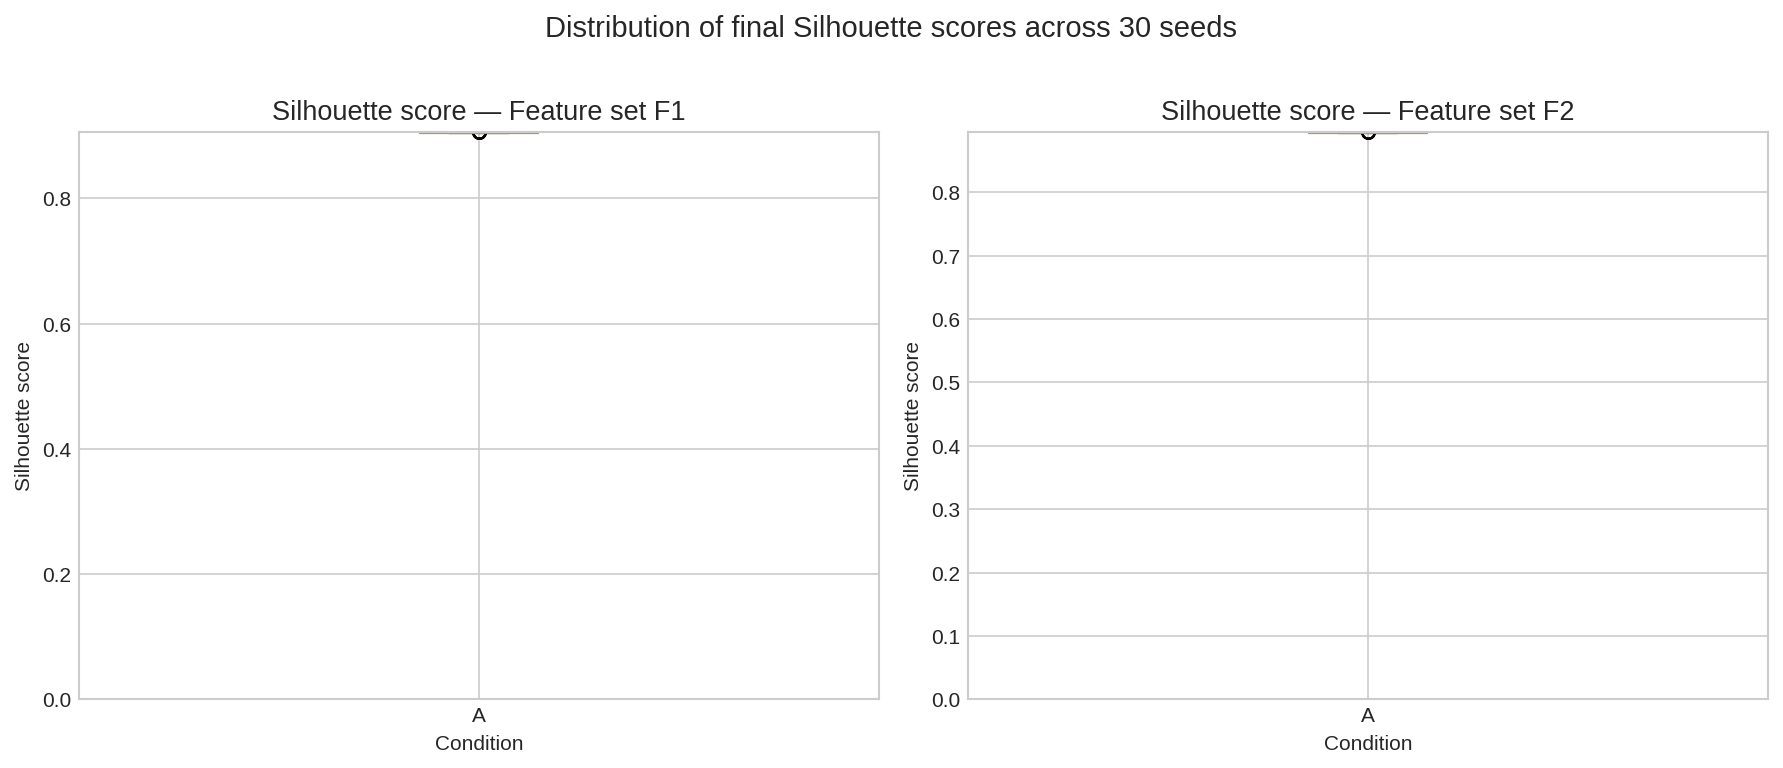
\includegraphics[width=\textwidth]{../runs/fig_silhouette_boxplot.png}
\caption{Final Silhouette score distributions across 30 seeds for each condition and feature set.}
\label{fig:boxplot}
\end{figure}

H1 compares Condition B against Condition A under F2, paired by seed. The median Silhouette improvement is $-0.0003$, with a 95\% bootstrap confidence interval of $[-0.0632, 0.0015]$. Across the 30 paired seeds, 13 show a positive B--A improvement, 15 show a negative improvement, and 2 are zero. Because the median improvement is not positive and the confidence interval includes zero, H1 is not supported.

\begin{figure}[H]
\centering
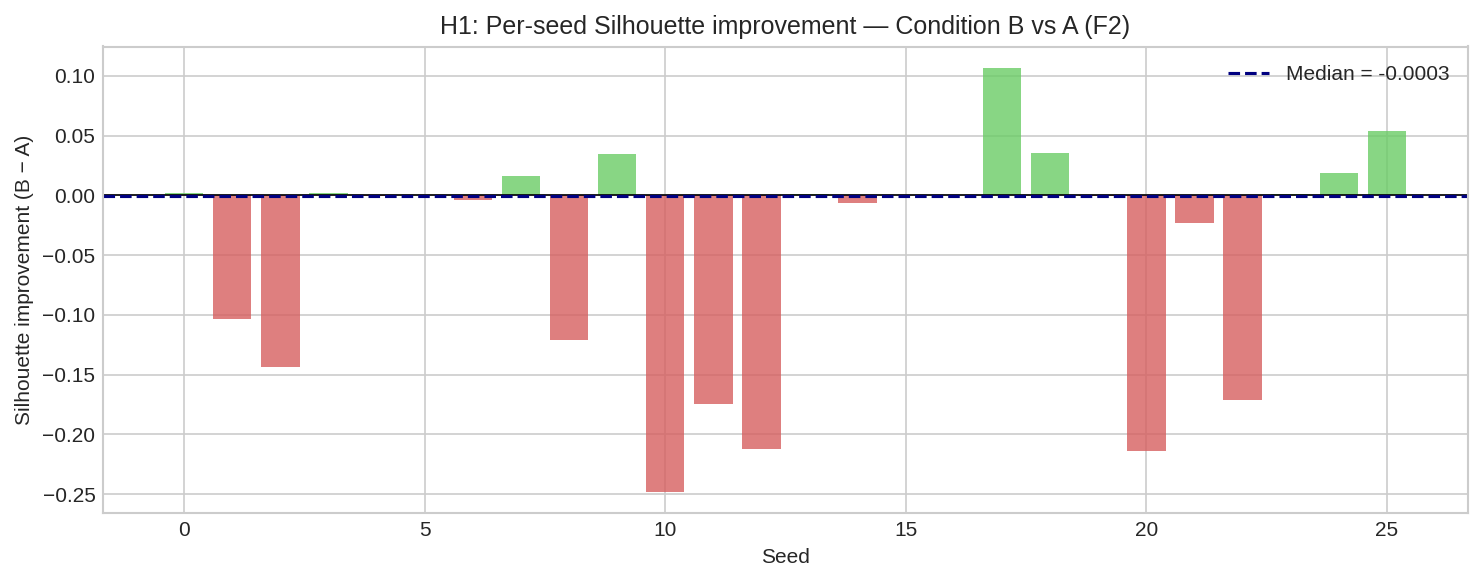
\includegraphics[width=0.95\textwidth]{../runs/fig_h1_improvement.png}
\caption{Seed-level H1 improvement under F2, computed as final Silhouette score for Condition B minus Condition A.}
\label{fig:h1}
\end{figure}

H2 is exploratory. It asks whether conversational refinement helps more under the richer feature set than under the location-only feature set. The observed median B--A improvement is 0 under F1 and $-0.0003$ under F2. The median difference between the F2 and F1 improvements is 0.0011, with a 95\% confidence interval of $[-0.0335, 0.0444]$. This means the project does not find clear evidence that the richer feature representation increases the benefit of conversational refinement.

\subsection{Exploratory Turn-Level Behavior}

The turn-level traces show why the conversational interface remains informative even when the final Silhouette result is cautious. Figure~\ref{fig:trajectory} shows the F2 trajectories for human and oracle refinement. Human refinement often changes the metric sharply early in the conversation and then stabilizes. Oracle refinement follows a smoother median path. For a political scientist, this trace is useful because it exposes how different refinement instructions pull the clustering toward different features and assumptions.

\begin{figure}[H]
\centering
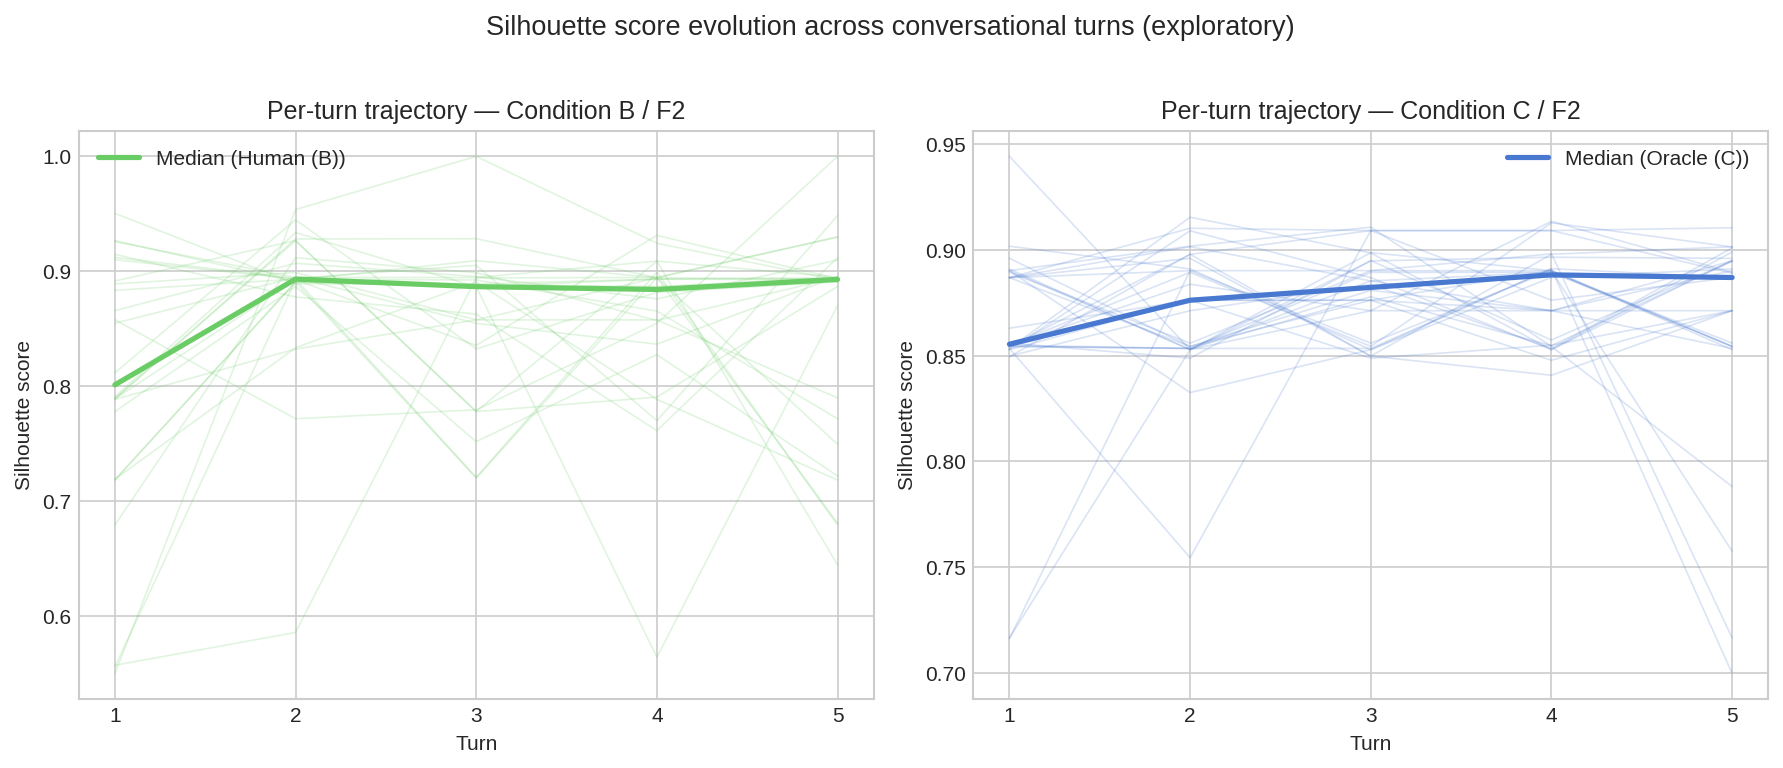
\includegraphics[width=\textwidth]{../runs/fig_turn_trajectory.png}
\caption{Exploratory F2 turn trajectories for human and oracle conversational refinement. Thin lines show seed-level runs; thick lines show the median trajectory.}
\label{fig:trajectory}
\end{figure}

The instruction taxonomy in Figure~\ref{fig:taxonomy} gives a complementary view. Human instructions under F2 are distributed across geographic, intensity, actor, balance, and generic categories. Oracle instructions are concentrated on geography and intensity. This supports one of the main practical interpretations of the project: conversational clustering is valuable not only as an optimizer, but also as a way for researchers to surface which dimensions of the dataset they are using to reason about political events.

\begin{figure}[H]
\centering
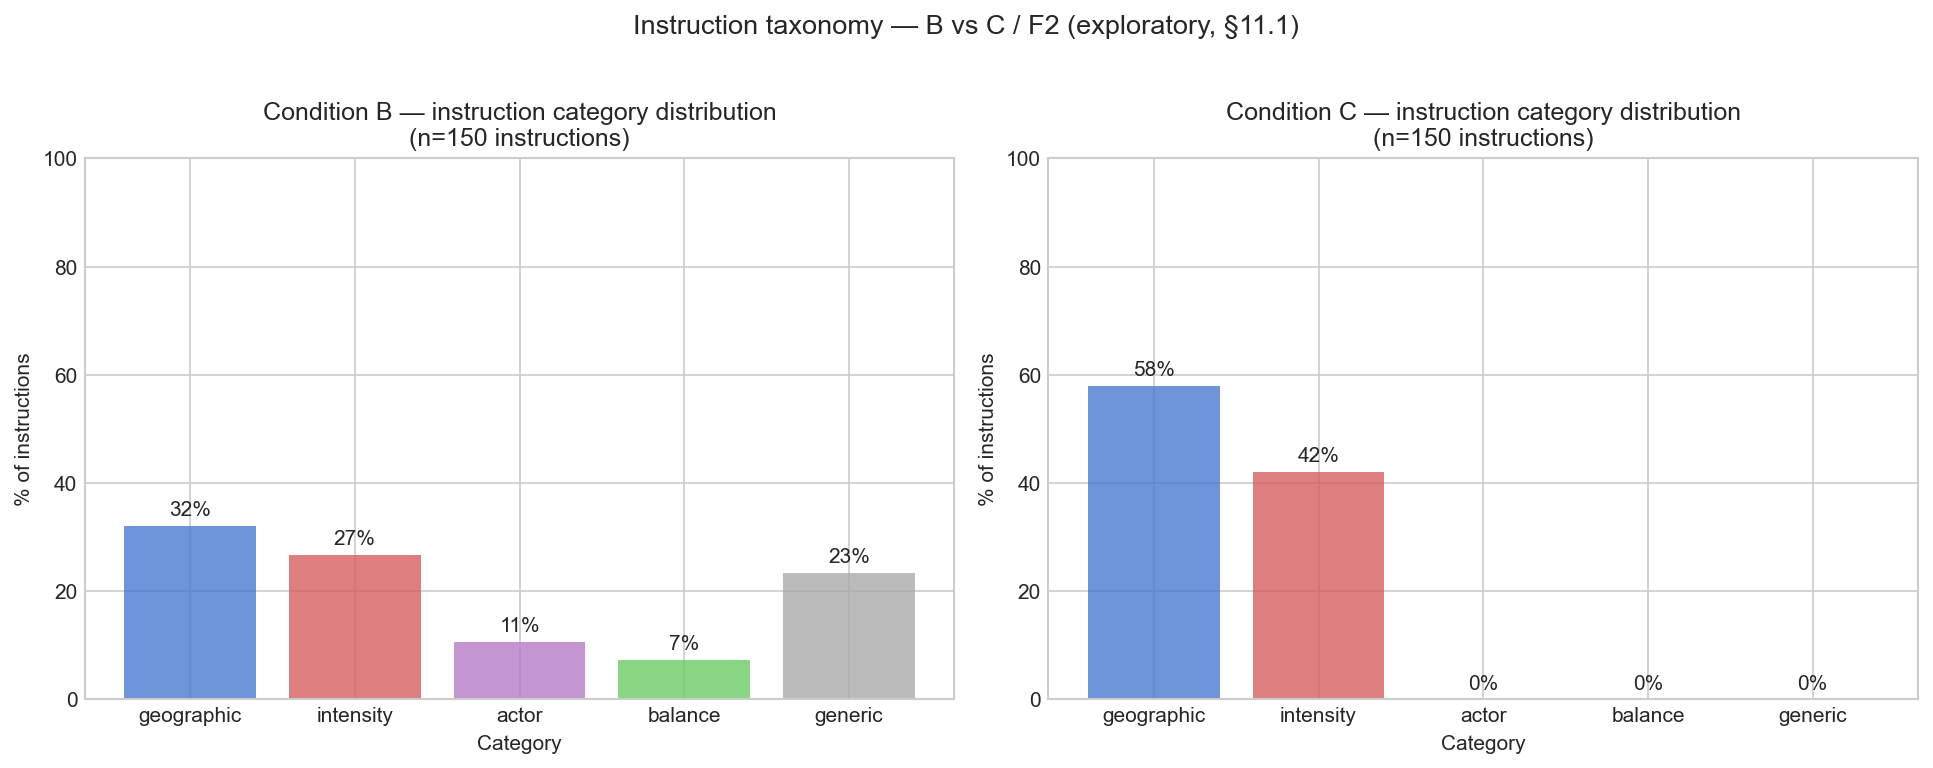
\includegraphics[width=\textwidth]{../runs/fig_instruction_taxonomy.png}
\caption{Exploratory instruction taxonomy comparing human and oracle refinement behavior under F2.}
\label{fig:taxonomy}
\end{figure}

\subsection{H3: Oracle Validity}

H3 tests whether the oracle can stand in for human judgment on cluster-quality comparisons. The result is negative. Human inter-rater reliability is low, with Krippendorff's $\alpha=0.13$. In the original displayed order, oracle-human agreement is 13 out of 20 pairs (65\%), with Cohen's $\kappa=0.22$ and Spearman's $\rho=0.24$.

The swap diagnostic is decisive. After the displayed A/B labels were swapped, the oracle kept the same displayed label in 19 out of 20 pairs, but kept the same underlying clustering in only 1 out of 20 pairs. This indicates displayed-label bias rather than stable judgment of the cluster content. Therefore, H3 is not supported.

\begin{table}[H]
\centering
\begin{tabular}{ll}
\toprule
Metric & Value \\
\midrule
Cluster-pair comparisons & 20 \\
Human raters & 5 \\
Krippendorff's $\alpha$ among humans & 0.13 \\
Original-order oracle-human agreement & 13 / 20 = 0.65 \\
Original-order Cohen's $\kappa$ & 0.22 \\
Original-order Spearman's $\rho$ & 0.24 \\
Same displayed label after swap & 19 / 20 \\
Same underlying clustering after swap & 1 / 20 \\
H3 status & Not supported \\
\bottomrule
\end{tabular}
\caption{H3 oracle-validity results from the committed H3 analysis outputs.}
\label{tab:h3}
\end{table}

\section{Discussion}

The results do not show that conversational refinement is a reliable way to improve internal clustering metrics on this dataset. The most plausible interpretation is tied to the nature of the data. The Russia-Ukraine GED sample is highly categorical, geographically concentrated, and dominated by a small number of event structures. In this kind of setting, feature-weight refinement can make the clustering more inspectable without necessarily improving a geometric metric such as Silhouette.

This distinction matters for political science use. The value of the workflow is not simply that it finds a better score. It gives researchers a structured way to ask what happens when geography, actor identity, event type, or fatality severity are emphasized differently. Even when the final metric does not improve, the interaction can help a researcher understand which features dominate the dataset, which assumptions are built into the clustering, and where automated groupings become politically hard to interpret.

The H3 result also clarifies the limits of automation. The oracle cannot be treated as a validated substitute for human cluster-quality judgment in this study. This does not make the oracle useless as an exploratory simulator, but it means that claims about interpretability should not rely on oracle preference scores alone.

\section{What We Can and Cannot Conclude}

We can conclude that the project built and ran a reproducible conversational clustering study over 180 logged runs, with fixed seeds, versioned configs, versioned prompts, and committed analysis artifacts. We can also conclude that, under the chosen metric and feature encodings, human conversational refinement did not clearly improve final Silhouette over the baseline under F2, and the richer feature set did not clearly increase refinement benefit.

We cannot conclude that conversational clustering is generally ineffective for political-event analysis. The study uses one conflict subset, one fixed $K$, one family of feature encodings, and internal clustering metrics that measure geometry rather than substantive interpretability. A stronger political-science conclusion would require richer feature representations, domain-expert evaluation, and possibly clustering methods designed for mixed categorical data.

\section{Limitations}

The first limitation is the absence of ground-truth cluster labels. Silhouette and Davies-Bouldin are useful internal metrics, but they do not directly measure whether a political scientist would find a cluster meaningful.

Second, the dataset is highly categorical and geographically concentrated. This makes the clustering task harder for k-means and may reduce the measurable benefit of conversational feature refinement.

Third, $K$ is fixed at 8. This protects comparability across conditions, but it does not test whether conversational refinement could help researchers choose a better number of clusters.

Fourth, H3 uses only 20 pairwise comparisons and five human raters. The low inter-rater reliability means that even the human reference signal is weak in this setting.

Finally, the oracle evaluation shows strong displayed-label bias. This limits the use of LLM judges as substitutes for human judgment in future versions of this workflow.

\section{Ethics}

The project uses a public academic conflict-event dataset. The data describes real violent events and fatality estimates, so the analysis is handled as sensitive political data even though it does not contain personal identifiers. The human rating task included a content-warning procedure and anonymized rater responses. No individual rater identities are reported.

The project also avoids presenting clusters as factual explanations of the conflict. The clusters are exploratory outputs produced from selected features and distance assumptions. They should be read as tools for analysis, not as authoritative political categories.

\section{Team Contributions}

Giacomo Vettore contributed to the data exploration, experimental execution, report/dashboard preparation, H3 documentation cleanup, and final synthesis. Daniele Notarangelo contributed to the initial study design and quality specification, repository structure, core clustering and logging implementation, Condition A and C execution, README/reporting materials, and figure updates. Jasnoor Singh contributed to the study-plan evolution, related-work synthesis, Condition B execution, H3 rating instrument and pair-generation materials, exploratory analyses, and H3 evaluation outputs. The final project reflects shared work across design, implementation, execution, analysis, and reporting rather than three isolated work streams.

\section{Conclusion}

This project tested conversational clustering as a study-first system for political conflict-event analysis. The main metric results are cautious: H1 is not supported, H2 is exploratory and inconclusive, and H3 does not validate the oracle as a substitute for human judgment. At the same time, the project demonstrates a reproducible workflow that lets political scientists interact with the feature structure of conflict data more directly. For highly categorical datasets like UCDP GED, conversational clustering may be most valuable as an interpretive and exploratory interface rather than as a guaranteed metric optimizer.

\begin{thebibliography}{99}

\bibitem{cohn2017}
Cohn, M., Chang, M., and Kauchak, D. Active learning for interactive cluster refinement. EMNLP, 2017.

\bibitem{choo2013}
Choo, J., Lee, C., Reddy, C. K., and Park, H. UTOPIAN: User-driven topic modeling based on interactive nonnegative matrix factorization. IEEE Transactions on Visualization and Computer Graphics, 2013.

\bibitem{amershi2014}
Amershi, S., Cakmak, M., Knox, W. B., and Kulesza, T. Power to the people: The role of humans in interactive machine learning. AI Magazine, 2014.

\bibitem{zhang2023}
Zhang, Y. et al. ClusterLLM: Large Language Models as a Guide for Text Clustering. EMNLP, 2023.

\bibitem{viswanathan2023}
Viswanathan, V. et al. Large Language Models Enable Few-Shot Clustering. arXiv:2307.00524, 2023.

\bibitem{grootendorst2022}
Grootendorst, M. BERTopic: Neural topic modeling with a class-based TF-IDF procedure. arXiv:2203.05794, 2022.

\bibitem{rousseeuw1987}
Rousseeuw, P. J. Silhouettes: A graphical aid to the interpretation and validation of cluster analysis. Journal of Computational and Applied Mathematics, 1987.

\bibitem{davies1979}
Davies, D. L., and Bouldin, D. W. A cluster separation measure. IEEE Transactions on Pattern Analysis and Machine Intelligence, 1979.

\bibitem{arbelaitz2013}
Arbelaitz, O., Gurrutxaga, I., Muguerza, J., Perez, J. M., and Perona, I. An extensive comparative study of cluster validity indices. Pattern Recognition, 2013.

\bibitem{zheng2023}
Zheng, L. et al. Judging LLM-as-a-Judge with MT-Bench and Chatbot Arena. arXiv:2306.05685, 2023.

\bibitem{chiang2023}
Chiang, C.-H., and Lee, H.-Y. Can large language models be an alternative to human evaluations? ACL, 2023.

\bibitem{guo2023}
Guo, Z. et al. Evaluating large language models: A comprehensive survey. arXiv:2310.19736, 2023.

\bibitem{sundberg2013}
Sundberg, R., and Melander, E. Introducing the UCDP Georeferenced Event Dataset. Journal of Peace Research, 2013.

\bibitem{croicu2017}
Croicu, M., and Sundberg, R. UCDP GED Codebook version 18.1. Uppsala Conflict Data Program, 2017.

\end{thebibliography}

\end{document}
